\documentclass[onecolumn,a4paper,amsmath,amssym,pre]{revtex4}
\usepackage{graphicx}% Include figure files
\usepackage{dcolumn}% Align table columns on the decimal point
\usepackage{subfigure}
\usepackage{bm}% bold math
\bibliographystyle{pf}
\usepackage{setspace}
\usepackage{fancyhdr}
\usepackage{amsmath}
\usepackage{color}
\usepackage{epstopdf}
\usepackage{booktabs}
\usepackage{xcolor}
\usepackage{hyperref}
\usepackage{ulem}
\usepackage[abs]{overpic}
\usepackage[document]{ragged2e}

\addtolength{\parskip}{0pt}
\addtolength{\floatsep}{0pt}
\addtolength{\textfloatsep}{0pt}
\addtolength{\abovecaptionskip}{0pt}
\addtolength{\belowcaptionskip}{0pt}
%\newcommand{\ra}[1]{\renewcommand{\arraystretch}{#1}
	\newcommand{\volume}{{\ooalign{\hfil$V$\hfil\cr\kern0.08em--\hfil\cr}}}
	
	
	
	
	\begin{document}
		
		
		\begin{tabular}{ r | l }
			\hline            
			\textbf{Manuscript Number}:& MS POF23-AR-08836R1 \\	
			\textbf{Title}: & Generating periodic vortex pairs using flexible structures\\
			%	\textbf{Revision title}: & Generating periodic vortex pairs using flexible structures \\  
			\textbf{Authors}:  & Gaurav Singh, Arahata Senapati, Abhishek Sharma, Arnab Atta and Rajaram Lakkaraju \\
			\hline  
		\end{tabular}
		\newline
		\vspace{0.5cm}
		%		\textcolor{red}{\textbf{Editor: Prof. Dr. Natalie Germann}}\\
		%		{\color{red}
			%			Dear Mr. Singh,
			%			
			%			We have determined that your submission falls well within the scope of Physics of Fluids and its chosen article type is appropriate. I have now heard from the referees regarding your manuscript, Flexible structures enhance fluid mixing in a channel flow; their reports are attached or below. As you will see, the reports point to issues that require clarification and revision.
			%			
			%			If you feel your revision can satisfy these reviewers, along with the editor commenting below, then please send your revised manuscript, a cover letter that includes an overview of your changes, and a separate point-by-point record for each referee. Upload each referee record as a separate file.
			%			
			%			Please upload two versions of the new submission. One, the "Article File," should be the final version of the revision and the other, uploaded as "Marked-Up Manuscript," should be the final version showing all changes from the former version. Do not provide a separate markup for each referee.
			%			
			%			When submitting your revision, please upload the source file for your revised manuscript. Figures must be embedded in the text and visible in the PDF. An author-generated PDF must also be provided since individual figure files are not being uploaded. You will also be asked to upload a highlight image that will be used in the table of contents if your manuscript is published. The highlight image should be a visually interesting figure representing your manuscript and may also be selected for the Cover Image. Further instructions will appear on the file upload screen.
			%			
			%			We expect to receive your revised manuscript by 09-Jan-2024. A later revision may be processed as a new submission, with a new received date and new referees.\\
			%			
			%			Sincerely,
			%			
			%			Univ.-Prof. Dr. Natalie Germann
			%			
			%			Deputy Editor, Physics of Fluids (IF 4.6, CS 6.4)
			%			
			%			Chair of Process Systems Engineering
			%			University of Stuttgart
			%			Böblinger Str. 78
			%			70199 Stuttgart
			%			Germany\\
			%			
			%			\color{black}{\textbf{Reply}: 
				
				To,
				
				The Deputy Editor,\\ 
				Physics of Fluids\\
				\par\null\par
				
				Thank you for considering the manuscript in the journal and providing valuable feedback from the reviewers. We carefully went through the reviewers' reports and appreciate the constructive comments. We want to express our gratitude to the reviewers for their thorough evaluation of the manuscript. We have addressed each of the reviewers' comments diligently in this rebuttal document, quoting each of them in full.
				\par\null\par
				We have incorporated the suggested modifications and improvements in the revised version of the manuscript. These improvements include additional analyses, more details on the explanation and a refinement in terms of  language and typographic errors. Overall, the review process has greatly enhanced the quality of the revised manuscript.	Furthermore, as per your recommendation, we have submitted two versions of the revised manuscript. One version includes the changes made, highlighted using a different font color, and the other is a clean, revised version for easier assessment.
				We express our gratitude for the guidance on the submission process and value the opportunity to contribute to the journal and match its high standards.\\
				\par\null\par
				\par\null\par
				Sincerely,\\
				
				Gaurav Singh\\
				(on behalf of all co-authors)\\
				Indian Institute of Technology, Kharagpur\\
				West Bengal -721302
				India
				%Dear Sir/Madam, \\
				%
				%
				%
				%Greetings. First, we sincerely thank you and the referees for strengthening our manuscript in many aspects and sharing the suggestions. The first referee recommended our manuscript with good words (like `the results and analysis seem compelling') and suggested we correct the language errors. \\
				%
				%
				%The second referee has praised our work by mentioning that `the physical discussion on the interplay between the oscillations and the tip generated vortices is quite interesting' and recommended a detailed revision of the manuscript by fixing the typos and careful choice of language. \\
				%
				%
				%
				%Our sincere apologies for the mentioned typo errors. Based on the referee reports, we have revised and resubmitted the manuscript in detail. Please find our rebuttals in this regard. Kindly accept our manuscript submission herewith. Thank you.				
				\newpage								
				%--------------------------------------------------
				\section*{\textbf{The first referee's comments and actions taken in that regard}}   
				
				\textcolor{red}{This article explores the improvement of fluid mixing in channel flows without a significant pressure drop by utilizing wall-mounted flexible plates as obstacles. Through fluid-structure-scalar interaction simulations, the study analyzes the oscillations of these plates, acting as vortex generators, to	enhance mixing. Evaluating mixing quality with metrics like the ’Mixing Index’ and ’Head Loss,’ the research compares various plate flexibilities and investigates the impact of pulsatile fluid inlets. Despite the article’s suitability for publication in PoF, the authors are encouraged to address the following comments in order to improve its quality.}\\
				
				\textbf{Reply}: Thank you very much for the thorough review and providing us a constructive feedback on our research article. We appreciate the recognition of the study's suitability for publication.  Your insights are invaluable, and we have made the necessary corrections and improvements based on your suggestions to enhance the overall quality of the manuscript.. We are grateful for your time and expertise in reviewing the article, and we look forward to the opportunity to refine and contribute to the field of fluid mixing in channel flows further.\\
				\par\null\par
				\textcolor{red}{\textbf{Major comments:}}
				
				
				\begin{enumerate}	
					
					\item \textcolor{red}{Regarding Figure 3(a), could you provide more details on the frequency and amplitude of the tiny tip oscillations of flexible plates that lead to the breakup of the jet-like flow? How exactly do these oscillations act as a source for perturbation, generating oppositely rotating vortex structures, and subsequently contribute to the stirring effect for fluid mixing downstream?}
					
					
					\textbf{Reply}: Our sincere appreciation for your inquiry and invaluable suggestions, we present a more detailed analysis of the dynamic behaviour of flexible plates exposed to fluid flow, with a focus on the frequency and amplitude of the tiny tip oscillations. We show that higher $Ca$ values lead to increased bending states. We have computed and scaled the mean bending amplitude for different $Ca$ as in the following Fig. \ref{fig:del_g_vs_Ca_steady}(a) (Fig 2 in the revised manuscript).
					\begin{figure}[h!]
						\begin{center}
							\begin{minipage}[c]{0.3\linewidth}	
								\centering	
								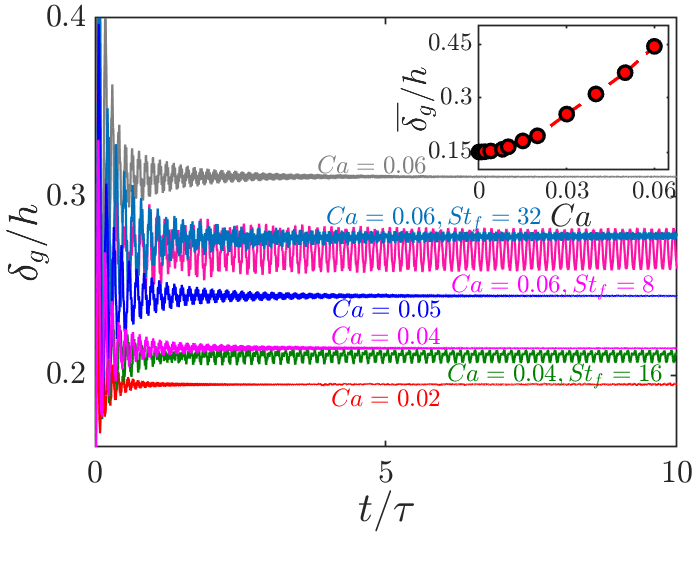
\includegraphics[width=1\linewidth]{Figures/gap_sig_4S_5S_5E_6D_6F_with amp.png}
							\end{minipage}  
							\begin{minipage}[c]{0.3\linewidth}	
								\centering
								\begin{overpic}[width=1\linewidth]{Figures/tipFreq/tip_freq_S_3D2.png} 
									\put(-149,-8){{\parbox{1\linewidth}{\footnotesize$(a)$}}}	
									\put(0,-8){{\parbox{1\linewidth}{\footnotesize$(b)$}}}	\put(165,-8){{\parbox{1\linewidth}{\footnotesize$(c)$}}}	
									
								\end{overpic}
							\end{minipage} 
							\begin{minipage}[c]{0.3\linewidth}	
								\centering
								\begin{overpic}[width=0.97\linewidth]{Figures/tipFreq/tip_freq_S2.png} 
								\end{overpic}
							\end{minipage} 
						\end{center}
						\vspace{-10px}
						\caption{$(a)$ Time history of gap-width between the tip of the two plates normalized by the channel height ($\delta_g/h$). $(b)$ Frequency spectra of the tip oscillations over time under steady inlet conditions for different $Ca$. $(c)$ Dominant frequency peaks identified from the spectra with $Ca$. }
						\label{fig:del_g_vs_Ca_steady}
					\end{figure}
					The inset figure highlights the mean gap amplitude ($\overline{\delta_g}$) increase with $Ca$ in steady inlet cases during the steady-state regime. However, under pulsatile inlet conditions, the gap oscillations or tip flutter amplitude exhibit a periodic regime aligned with the inlet conditions. The intermittent inertia from the inlet results in lower mean bending despite the periodic flutter. We further show the frequency characteristics of tip oscillations by conducting a Fast Fourier Transform (FFT) analysis of the time-domain data in Fig. \ref{fig:del_g_vs_Ca_steady}(b). The frequency spectra are non-dimensionalized into tip Strouhal number ($St_{tip}$), expressed as $\frac{f_{tip}h}{U}$. In Fig. \ref{fig:del_g_vs_Ca_steady}$c$, the identified $St_{tip}$ associated with maximum energy content ($E$) reveals dominant peak frequencies representing primary oscillation modes. We found that the highest tip flutter frequency occurs at $Ca=0.03$, and beyond this critical value, a reduction is observed. This intricate interplay of fluttering modes contributes to the generation of multiple vortices, creating a complex flow field. The text emphasizes that this complexity is significantly influenced by plate flexibility, highlighting the importance of considering fluid-structure interaction dynamics in flexible plate scenarios compared to rigid plate cases.
					
					
					We have incorporated the above details on the bending amplitude and tip oscillation frequency of flexible plates in Figure 2 of the revised manuscript and are now presented more comprehensively. Furthermore, in the results section of the revised manuscript, we have expanded the discussion on how these oscillations serve as a source for perturbations, generating oppositely rotating vortex structures. The detailed impact of these vortex structures on the stirring effect for fluid mixing downstream is now discussed more explicitly in the discussion of the results of Figure 3. We hope these additions enhance the clarity and understanding of the fluid-structure interaction dynamics in the manuscript. 
					
					\item \textcolor{red}{In Figure 3(b), when discussing the scalar concentration field, what is the critical downstream location in the rigid plate case where the jet-like flow oscillates, leading to the detachment of vortex structures and, eventually, mixing of scalar fields?}
					
					\textbf{Reply}: Our sincere apologies for the oversight of this critical detail. We have now added a coordinate axis to the figure 3(b), providing a clear reference for downstream locations. In the respective paragraph discussing the scalar concentration field, we have explicitly mentioned the critical downstream location, i.e. `$x\approx5h$' in the rigid plate case where the jet-like flow oscillates, leading to the detachment of vortex structures and eventual mixing of scalar fields. We appreciate your feedback in guiding us to make these improvements.
					
					\item \textcolor{red}{What specific characteristics or parameters determine the delayed mixing observed in the rigid plate case compared to the flexible plate case?}
					
					\textbf{Reply}: Thank you for your kind inquiry and keen interest on the topic. The mixing in the flexible plates case is observed early in the channel compared to rigid plates case which shows gradual increase in $MI$. As the flow passes through the gap between the rigid plates the shear layer extends longer in the downstream direction which forms a jet-like flow. Upon a critical length, this jet destabilises and begins to oscillate generating vortex structure which induce inter-mixing of the scalar fields. This jet length is longer in rigid plates case in comparison to flexible plates case where, the emanating jet breaks up immediately due to the plates' oscillation. Thus, the resulting flow features, especially the jet length can be identified as the discernible characteristics for delayed mixing in the rigid plate case. We have included these details in the revised manuscript while discussing the vortex structures in Fig. 5(a).
					
					\item \textcolor{red}{Explain how the vorticity dynamics, as illustrated in Figure 5 for $Ca = 0.04$ with $St_f = 1-32$, differ under pulsatile inlet conditions compared to steady inlet conditions?}
					
					
					\textbf{Reply}: We sincerely apologise for the lack of explanation regarding the Figure 5. We thank the reviewer for allowing us the opportunity to rework on the details. In response, we have presented following insights based on the instantaneous vorticity contours in the Figure.
					
					\textit{Upon careful examination of Fig. 5, we find that the pulsatile inlet flow interacts with the oscillations of the flexible plates, giving rise to vortex structures in varying numbers. These vortices arrange themselves in an alternating fashion at later times and persistently roll, contributing to local mixing as they advect downstream. The size of these rolling vortices gradually diminishes due to the influence of viscosity. Particularly noteworthy is the observation that cases with $St_f = 1-16$ generate even more organized vortices and achieve a delayed steady state compared to steady inlet conditions. However, in the case of $St_f = 32$, the vorticity patterns closely resemble those of the steady inlet scenario and also similar mixing patterns can be observed. This observation suggests that, for higher values of $St_f$, the vorticity dynamics and resulting mixing patterns under pulsatile inlet conditions converge towards those observed in the steady inlet case. The interplay between flow pulsation and plate oscillations continues to shape the vorticity structures, emphasizing the intricate relationship between inlet conditions, plate flexibility, and ensuing flow dynamics}   
					
					In the revised manuscript, we have included the above detailed information in the relevant section concerning Figure 5, explicitly stating how the vorticity dynamics differ between pulsatile and steady inlet conditions. 
					
					\item \textcolor{red}{Additionally, what insights can be derived from Figure 6 regarding the Mixing Index (MI) and Head Loss (HL) along the downstream location, especially in the case where the flow inlet occurs at $St_f = 2$?}
					
					\textbf{Reply}: Our sincere thanks for your keen observation on the manuscript. We appreciate the opportunity to provide additional insights into the Mixing Index (MI) and Head Loss (HL) along the downstream location.
					
					\textit{Upon quantifying the corresponding mixing index $MI$ and head loss $HL$, we show these metrics along the downstream location in Fig. 6. $MI$ for pulsatile inlet cases show a steeper increase early in the channel compared to the steady inlet case. The flow exiting through the gap between the plates in pulsatile inlet cases show increased flow agitation near the plates due to the interaction between flow pulsation and tip oscillations. This interplay breaks up the emanating jet-like flow and releases various scales of vortices that move laterally and further interact, merge, and advect to influence the $MI$. This behavior is attributed to the interplay between flow pulsation and the tip oscillations of the flexible plates. The emanating jet-like flow breaks up near the plates, generating various scales of vortices that contribute to enhanced mixing. In the case with $St_f=2$, we observe the steepest shoot in the $MI$ next to the plates as the flow and structure oscillations intensifies due to the multiple modes involved. In contrast, the steady inlet case primarily relies on the oscillations of flexible plates for flow agitation and subsequent mixing, resulting in a longer jet length. However, at $x=8h$ downstream, the $MI$ results converge for all cases, indicating that the mixing characteristics stabilize further along the channel. This convergence suggests that, despite differences in the mixing process initiation, the mixing index reaches a consistent state at this specific downstream location. The corresponding $HL$ values are higher immediately next to the flexible plates in the pulsatile inlet conditions, reflecting the increased flow agitation near the plates due to the interaction between flow pulsation and tip oscillations. This is because at low inlet pulsation the flow exhibit lower flow inertia which results in a diminishing effect of the periodic inlet at longer downstream locations when computing steady-state statistics. }
					
					In response to your inquiry, we have included these additional details in the relevant section, elaborating on the insights derived from Figure 6 regarding the Mixing Index (MI) and Head Loss (HL) along the downstream location. The updated manuscript provides a more thorough discussion of the flow features, highlighting the specific characteristics observed in the Mixing Index and Head Loss statistics along the downstream location. 
					
					\item \textcolor{red}{Provide further details on how the Coefficient of Performance (CoP) varies across different $Ca$ and $St_f$ cases, as shown in Figure 7(b).}
					
					\textbf{Reply}: Our sincere apologies for not clearly mentioning details in the earlier submission. In the revised manuscript, we have included the following additional details in the relevant section to elaborate on how the Coefficient of Performance ($CoP$) varies across different $Ca$ and $St_f$ cases, as shown in Figure 7(b). 
					
					\textit{In Fig. 7(b), the observed CoP trends reveal important features in the relationship between plate flexibility, pulsatile inlet conditions, and the resulting mixing performance. For lower $Ca$ values in the range of $0-0.02$, the mixing performance does not exhibit significant improvement. This is attributed to the higher Head Loss $(HL)$ in the flow caused by less flexible plates, counteracting the potential benefits of plate oscillations. Conversely, as $Ca$ increases beyond $0.02$ i.e. highly flexible plates, the reduction in $HL$ becomes more pronounced due to the larger gap opening between the plates. Additionally, the oscillations of the flexible plates induce vortex shedding, contributing to enhanced Mixing Index $(MI)$ compared to rigid plate cases. The curve clearly indicates that the flexible plates indeed offer superior mixing performance. However, pulsatile inlet conditions do not yield a substantial improvement in overall mixing performance compared to steady inlet cases. This is due to the diminishing effect of periodic inlet conditions at longer downstream locations during steady-state conditions. Moreover, higher $HL$ values in cases with lower $St_f$ negatively impact mixing performance, resulting in marginally lower net $CoP$. Instead, the cases with lower $St_f$ $(<32)$ show adverse mixing performance and it is recommended to use steady inlet conditions. However, at $St_f = 32$  i.e. with higher pulsatile inlet conditions, the mixing performance closely resembles that of steady inlet cases, demonstrating a similar $CoP$ but achieves a marginally better $CoP$ compared to the steady inlet case. This indicates that the interplay between plate flexibility and pulsatile inlet conditions when under similar flow inertia results in enhanced $CoP$.}
					
					The updated manuscript now provides a more thorough discussion, offering insights into the specific trends and variations observed in the $CoP$ for different combinations of $Ca$ and $St_f$. Thank you very much for your feedback and guidance in improving the manuscript.
					
					
					\item \textcolor{red}{How do the flexible plates contribute to better mixer performance, and why does the pulsatile inlet not result in a substantial improvement in overall mixing performance, despite the observed benefits of increased flexibility?}
					
					\textbf{Reply}: Thank you for very much your thoughtful inquiry. We have included the following additional details in the summary section in the revised submission to explain how flexible plates contribute to better mixer performance and why the pulsatile inlet does not substantially improve overall mixing performance despite the observed benefits of increased flexibility.
					
					\textit{The flexible plates induce flow transition early in the channel by introducing vortex generation. The flexibility of the plates allows for dynamic interactions with the flowing fluid, promoting vortex shedding and enhancing the mixing process. This effect contributes to improved mixing performance compared to the rigid plate case.
					On the other hand, in the case of a pulsatile inlet, while there are benefits associated with the flexibility of the plates, the overall mixing performance is not substantially improved. This is attributed to the intermittent flow inertia caused by the pulsatile flow condition which impart relatively lower agitation in the flow, and additionally, the effect of pulsation tends to get washed away at longer downstream locations at steady-state times}.
					
					We appreciate your feedback and hope these additional details provide a more comprehensive explanation of the observed phenomena. 
					
					\item \textcolor{red}{It is not clear to me, what specific factors make $Ca = 0.06$ with $St_f = 32$ stand out as the optimal configuration for fluid mixing in your setup?}
					
					\textbf{Reply}: Thank you for your inquiry regarding the optimal configuration for fluid mixing in our setup. In our investigation, we observed that the configuration with $Ca=0.06$ exhibited increased mixing performance and reduced head loss compared to other configurations. The higher plate flexibility at $Ca=0.06$ contributes to enhanced tip oscillations, promoting vortex generation and effectively disrupting the flow, improving the mixing efficiency.
					Regarding the pulsatile inlet conditions, we acknowledge that, in general, pulsatile inlets did not contribute significantly to the overall mixing performance. However, the case with $St_f=32$ demonstrated a marginally significant mixing performance than the steady inlet condition. This marginal improvement is attributed to the higher flow inertia compared to the low $St_f$ cases, which feature intermittent inlet inertial forces. The $St_f=32$ case exhibit close resemblance with the steady case but with additional vortex shedding, which enhances the overall mixing performance.			
					We have now included a relevant discussion in the revised manuscript, highlighting the specific features of $Ca=0.06$ with $St_f=32$ that contribute to its prominence in terms of mixing efficiency.
					
					\item \textcolor{red}{The potential avenues for future research to address the limitations of the current study, particularly in terms of the geometric design of the channel mixer. How might more complex or realistic channel geometries be incorporated to further enhance the applicability and insights gained from your findings?}
					
					\textbf{Reply}: We appreciate your acknowledgement of the potential avenues for future research to address the limitations of our current study, particularly in terms of the geometric design of the channel mixer.
					In response to your question, we have included a paragraph in the summary section that discusses possible avenues for incorporating more complex or realistic channel geometries to enhance the applicability and insights gained from our findings. We suggest exploring geometric modifications such as introducing wall-mounted plates at an offset, varying the flexibility of each plate, and considering a tandem series of such plates. These modifications can provide a more nuanced understanding of the fluid-structure interaction and mixing efficiency in diverse practical scenarios.
					We hope that these proposed future research directions adequately address your inquiry.
				\end{enumerate}	
				
				\newpage	
				
				\section*{The second referee's comments and actions taken in that regard} 
				
				\textcolor{red}{Subject of the paper: The authors study the enhancement of mixing in a rectangular (2d) channel. To this end, they use flexible (elastic) obstacles at the side walls. The authors consider two kinds of basic flow: steady flow and oscillatory flow at the inlet. The numerical procedure looks fine, the results seem reliable. In this sense, the paper is perfectly suitable for PoF with new ideas in a very interesting field with applications in technology. The title reflects the scope of the paper, the language is clear.}\\
				
				\textcolor{red}{\textbf{General comments:}}\\
				\begin{itemize}
					\item \textcolor{red}{Organization of the text in Section 2, Mathematical Formulation and Computational setup: The authors should begin first with the mathematical-physical formulation of the problem, including boundary conditions and after that continue with the mathematical-numerical solution procedure. The authors jump to and fro between the formulation and the solution procedure. This causes unnecessary confusion.
					}
					
					\textbf{Reply}: Thank you for your valuable feedback and guidance on strengthening the manuscript structure. We have revised Section 2, `Mathematical Formulation and Computational Setup, ' to enhance the organization of the text and ensure a logical flow. The updated manuscript now begins with a clear presentation of the physical problem, providing a detailed description of the two-dimensional channel geometry, the placement of flexible plates, and the overall setup. Following this, the mathematical formulation is systematically presented, covering the governing equations for fluid and structure, boundary conditions, and the introduction of the scalar concentration field.
					After establishing the physical and mathematical foundations, the numerical strategy is introduced in a separate subsection, outlining the numerical methods employed for solving the coupled fluid-structure interaction problem.
					
					Lastly, the parametric definition is presented in a paragraph clearly detailing the varied parameters, such as Cauchy Number and Strouhal Number. The changes made have been highlighted in the marked-up manuscript for easy reference. These revisions address the concerns regarding the organization of the text and reduce any unnecessary confusion.
					
					\item \textcolor{red}{Numerical domain: Influence of the backward effect of the outer (outlet) boundary on the velocity field. Check this by extending the domain.}
					
					\textbf{Reply}: Thank you very much for your query. We appreciate the concern regarding the potential influence of the outlet boundary on the velocity field. In the updated manuscript, we have explicitly mentioned that all metric computations are conducted at a streamwise location of $x=8h$ at a steady state out of the total channel length of $14h$. This choice is made to mitigate the effects of reflective boundary conditions and ensure that the properties of interest are sufficiently cushioned out before reaching the channel exit. Therefore, the numerical domain has been specifically selected to avoid the backward effects of the outer (outlet) boundary on the results.
					\\
				\end{itemize}
				
				\textcolor{red}{\textbf{Specific comments:}}\\
				
				\begin{enumerate}
					\item \textcolor{red}{Karman vortex street:
						The results in the figures remind me of the Karman vortex street. The authors should discuss this issue in detail.}
					
					\textbf{Reply}: Thank you for your insightful observation and comment. We appreciate your keen interest in our work. We want to clarify that although the flow field in the figures may bear a resemblance to a von Kármán vortex street, it is not a typical von Kármán vortex street formation.
					
					In our study, the flow initiates by emanating through the slit in a jet-like manner. Subsequently, the flow rolls up on either side, forming a co-rotating vortex pair. As the flow progresses, the effects of the boundary walls come into play, leading to a rearrangement of the flow in an alternating fashion. This phenomenon may superficially resemble transient vortex shedding akin to a von Kármán vortex street, but in the present case, vortex shedding off each plate's tip is simultaneous, which simply arranges itself in an alternate fashion due to the oscillation of jet-like flow under the boundary effects.
					
					To provide a more detailed discussion, we have explicitly addressed the specific flow dynamics, emphasizing that the observed alternating pattern results from boundary wall effects interacting with the initially formed vortex pair. This clarification is incorporated into the revised manuscript, ensuring a more accurate representation of the flow characteristics.
					
					\item \textcolor{red}{I want to draw the attention of the authors to some further interesting and most relevant literature regarding the idea "manipulation of the flow with obstacles":}
					
					\begin{enumerate}
						\color{red}{	\item Manipulation of the flow in channels:
							Massive stabilization of gravity-driven film flows with corrugated side walls.
							
							Kögel, A and Aksel, N,
							Nov 2018 PoF
							30 (11)
							
							\item  Stability of the channel flow - new phenomena in an old problem.
							
							Kögel, A and Aksel, N,
							Mar 2020 Acta Mechanica,
							231 (3) , pp.1063-1082
							
							\item Manipulation of the flow in pipes:
							Gravity-driven film flow inside an inclined corrugated pipe: An experimental investigation of corrugation shape and tip width.
							
							Kuehner, JP, Dec 2022 PoF, 34 (12)
							
							\item The effect of substrate amplitude and wavelength on gravity-driven film flow inside an inclined corrugated pipe
							Kuehner, JP; Lee, MR; (...); Kutelak, LO
							Nov 2021 PoF
							33 (11)
							
							\item Natural or man-made mixing in the environment with obstacles (very important nowadays: e.g. gravity-driven free surface flows in nature, flooding etc.)
							
							Pattern formation and mixing in three-dimensional film flow
							Heining, C; Pollak, T and Aksel, N
							Apr 2012 PoF
							24 (4)}
						
					\end{enumerate}
					
					\textcolor{red}{Comparisons with the above given literature:\\	
						Can the authors learn something from these papers for their paper?\\
						- Novelty compared to the reference [62]:\\
						This must be explained very clearly in the beginning.}
					
					\textbf{Reply}:
					Thank you very much for bringing these relevant literature references to our attention. We find these works are very relevant in terms of geometric variations and offer valuable learnings about flow manipulation techniques, addressing stability, pattern formation, and mixing in different configurations. %We have carefully reviewed the mentioned papers, specifically those related to the manipulation of flow in channels and pipes. %However, a one-to-one comparison may not be possible because of the fundamental nature of the problem, as these include open channel film flows that deal with gravity, surface tension and boundary flows.
					We acknowledge the importance of these works, and their relevance to our study is now explicitly discussed in the introduction section, which draws connections between our work and the insights gained from these studies. We appreciate the reviewer's guidance, and incorporating these discussions will contribute to a more informed and well-contextualized presentation of our research.
					
					Regarding novelty compared to the reference [62] in the manuscript (\cite{Self2019}), we have explained how this work is an extension to the same work with further investigation which delves deeper into the scalar concentration mixing concerning flexibility and pulsatile flow inlet. We have included the following text in the introduction section in the revised manuscript.
					
					\textit{This geometrical configuration builds upon our earlier work [62], where we investigated the scaling of energy dissipation in a channel flow featuring flexible obstacles across different Reynolds numbers. The previous study highlighted that flexible plates contribute to early flow transition and identified an optimized geometric setup. This current work utilizes the established geometric configuration to explore mixing in the context of scalar concentrations and pulsatile flow inlet, introducing a novel aspect to our research. We focus on an approach to inertial mixing that capitalizes on the flow-induced bending and oscillations of the flexible plates to enhance mixing.}
					
					
					\item \textcolor{red}{Enhancing the mixing quality:	Can multiple rigid or flexible obstacles increase or even decrease the quality of mixing? A short discussion would be very helpful. Can the authors give a speculative discussion on 'overall geometrical optimization'?}
					
					\textbf{Reply}: Our sincere thanks to you for taking interest into the research and presenting novel ideas which may eventually turn out as potential future works. In response to your query regarding multiple obstacles, we can speculate that in the present range of $Re$ ($\approx500$), multiple rigid or flexible obstacles in the channel shall consume much inlet energy in their deformation and also hamper pressure head, thereby reducing the net mixing performance. However, such a work could be a valuable extension to the present work, and we shall indeed consider formulating a relevant problem as an extension to this work. 
					
					We also propose a geometric variation with two wall-mounted plates as in the present case but with an offset and each of different structural properties. We acknowledge that the interaction between these obstacles may lead to either an enhancement or a reduction in fluid mixing, depending on the specific geometric arrangement. Further research in this direction is warranted to explore the intricate dynamics of such configurations and unveil the possibilities for overall geometrical optimization.
					
					As per your suggestion, we have incorporated a new paragraph at the end of the summary section to address the potential influence of multiple rigid or flexible obstacles on the mixing quality. 
					
					\item \textcolor{red}{What is the dependence of the Re number of the basic flow on the mixing quality? What would happen when varying the Re number e.g. from creeping flow to inertial flow? Stages?
						. (I do not expect a precise answer because the 'maximum-optimum' is beyond any consideration with so many parameters involved in the problem.)}
					
					\textbf{Reply}: We appreciate the importance of investigating the dependence of Reynolds number (Re) on mixing quality. The Reynolds number is indeed a crucial parameter that can significantly influence the mixing performance. In our previous work \cite{Self2019}, we have conducted a similar investigation where we correlated viscous diffusion with increasing Re. This provided valuable insights into the relationship between Reynolds number and energy dissipation potential mixing characteristics. Upon increasing the $Re$ in the range $200-3200$, the increased inertia contributed towards higher viscous energy dissipation in the downstream by cascading vortices into smaller structures, which in turn should increase fluid mixing for a setup as in the present work. In another work with J-shaped rigid baffles channel mixer \cite{Lin2007}, authors have investigated two scalar fields mixing in steady flow with different $Re$ ranging from $5-350$. They concluded towards an evident increase in mixing performance with increasing $Re$.
					
					Building on this foundation, we acknowledge that extending the current study to explore the effects of Reynolds variation on mixing quality of could be an interesting and informative investigation. We shall seriously consider it for future extensions of our investigation, and it should be a valuable addition to our research.
					
					\item \textcolor{red}{What can we learn from Fig.10? The curves are too scattering. Is it physically correct to connect the points?}
					
					\textbf{Reply}: Our sincere apologies for overseeing this observation regarding Fig. 10. We appreciate your attention to detail, as it is indeed incorrect to connect the scattered data points. In the updated manuscript, we have now refrained from connecting the data points. The scattering of curves in this figure is a result of the variability in the data points, and the current investigation is not indicative of any physical connection between them. 	
					Figure 10 is provided in the appendix section solely to complete the $St_f$ labelling of Figure 7(a). The intention is to offer a reference for the various curves shown in Figure 7(a), and any explanation of the scattered data points is beyond the scope of the current work and demands an extensive investigation by taking care of several other factors which we have planned to explore in our future studies.
					
					\item \textcolor{red}{The equations in the paper must have numbers so that they can be cited in the text.}
					
					\textbf{Reply}: Our sincere apologies for the absence of equation numbers in the manuscript. We have made the necessary corrections in the updated version. Each equation in the paper is now assigned a number in sequence, allowing for proper citation in the text. We appreciate your attention to detail, and this adjustment aims to enhance the clarity and referenceability of the mathematical content in our manuscript.
					
					
					\item \textcolor{red}{Typos:
						page 1, abstract: efficacy
						page 3, right column: Schimdt number
						Check the whole paper!}
					
					\textbf{Reply}: Thank you for bringing these typos to our attention. We sincerely apologize for any oversight in the initial submission. In the updated manuscript, we have corrected the mentioned typos and checked the manuscript to our best. We appreciate your thorough review and feedback and submitting an even more refined version of the manuscript. 
				\end{enumerate} 
				
				\vspace{1cm} 
				Yours sincerely,\\
				\vspace{0.1cm}
				Gaurav Singh \\
				\today \\
				IIT Kharagpur, India.
				
				\begin{thebibliography}{100} % 100 is a random guess of the total number of
					%references
					\bibitem{Self2019} Singh, Gaurav and Lakkaraju, Rajaram, ``Wall-mounted flexible plates in a two-dimensional channel trigger early flow instabilities", \emph{Phys. Rev. E}, American Physical Society, Vol. 100, 2 pp. 023109, Aug 2019.
					\bibitem{Lin2007} Lin, Yu-Cheng, Chung, Yung-Chiang and Wu, Chung-Yi, ``Mixing enhancement of the passive microfluidic mixer with J-shaped baffles in the tee channel", \emph{Biomedical Microdevices}, Vol. 9, 2 pp. 215-221, Apr 2007.
				\end{thebibliography}
				
			\end{document}